% =============================================================================
% presentacion_comparacion_2012.tex — Beamer: reproducción figura-por-figura
% de Gutiérrez et al. (2012), Sección 4, y mejoras hechas sobre ella.
% Para reunión con Gonzalo (julio 2026).
% Compilar (desde docs/reunion_gonzalo/): pdflatex presentacion_comparacion_2012.tex
% Fuentes: docs/manuscrito/comparacion_energias_2012.tex
%          docs/manuscrito/comparacion_figuras_2012.tex
%          docs/manuscrito/figuras_2012_original/ (imágenes extraídas del capítulo)
% =============================================================================
\documentclass[11pt,aspectratio=169]{beamer}

\usetheme{Madrid}
\usecolortheme{seahorse}
\setbeamertemplate{navigation symbols}{}
\setbeamertemplate{footline}[frame number]

\usepackage[utf8]{inputenc}
\usepackage[T1]{fontenc}
\usepackage[spanish,es-nodecimaldot]{babel}
\usepackage{amsmath,amssymb}
\usepackage{graphicx}
\usepackage{booktabs}

\newcommand{\eps}{\varepsilon}
\newcommand{\lammps}{\textsc{Lammps}}

\title[Reproducción 2012]{Reproduciendo Gutiérrez et al.\ (2012)\\
\large Comparación de energías y figuras, y qué mejoramos}
\author[F. Wasaff]{Felipe Wasaff\\
\footnotesize reunión con Gonzalo Gutiérrez}
\institute[IMA-PUCV]{Instituto de Matemáticas, PUCV}
\date{Julio 2026}

\begin{document}

% -----------------------------------------------------------------------------
\begin{frame}
\titlepage
\end{frame}

% -----------------------------------------------------------------------------
\begin{frame}{Por qué reproducir antes de extender}
\begin{itemize}
    \item Todo el proyecto nuevo (barrido en $N$, orientaciones,
    $\alpha_{\rm surf}$, $N_c^{\rm ef}$) se apoya en que
    \texttt{in.bounce\_reprod} resuelve \textbf{el mismo problema} que la
    Sección~4 del capítulo 2012 (``Bouncing of a ball over a surface'').
    \item Antes de confiar en las extensiones, confirmamos esto
    \textbf{figura por figura}: instantáneas, alturas de rebote,
    $g(r)$ de la bola, y evolución temporal de las energías.
    \item Esta charla muestra esa comparación y las tres mejoras
    concretas que salieron de hacerla.
\end{itemize}
\medskip
\begin{alertblock}{En una frase}
La física coincide, panel por panel, con un código de MD completamente
distinto (\lammps{} vs.\ \emph{Las Palmeras MD}) --- y al reproducir la
receta exacta del capítulo encontramos un problema medible que motivó
gran parte del resto del proyecto.
\end{alertblock}
\end{frame}

% -----------------------------------------------------------------------------
\begin{frame}{Las mismas ocho energías, reorganizadas en cuatro canales}
\small
\begin{tabular}{lll}
\toprule
Gutiérrez 2012 & Este estudio & \\
\midrule
$K_B=\tfrac12M_B\|\mathbf V_{\rm CM}^B\|^2$ &
    $\alpha_{\rm cm}=h_1/h_0^{\rm ef}=e_1^2$ & (equivalentes) \\
$T_B=\sum_{\rm bola}\tfrac12m_i\|\mathbf v_i-\mathbf V_{\rm CM}^B\|^2$ &
    $\alpha_{T_B}=T_B^{(1)}/E_0$ & (idéntica) \\
$V_B=\sum_{\rm pares\ bola}V(r)$ &
    $\alpha_{\Delta V_B}=(V_B^{(1)}-V_B^{(0)})/E_0$ & (idéntica, restamos cohesión) \\
$U_c=\sum_{\rm pares\ bola-sup.}V(r)$ &
    --- (nulo en el apogeo) & \\
$K_S,T_S,V_S$ &
    $\alpha_{\rm surf}=\Delta(K_S+V_{\rm surf})/E_0$ & (canal nuevo, ver siguiente) \\
\bottomrule
\end{tabular}
\bigskip

\textbf{Diferencia clave:} el capítulo grafica las 8 energías en función
\emph{continua} del tiempo (su Fig.~9); nosotros las evaluamos en un
único instante --- el primer apogeo --- y las normalizamos por $E_0$, para
poder comparar 210 corridas con un solo número por canal en vez de
210 curvas.
\end{frame}

% -----------------------------------------------------------------------------
\begin{frame}{Ecuaciones desarrolladas (I): son la misma suma de pares}
\small
Sea $\mathcal B$ la bola y $\mathcal S$ la superficie, $r_{ij}=\|\vec r_i-\vec r_j\|$.
Sustituyendo el potencial LJ ($c=1$ mismo tipo, $c=0$ bola--superficie):
\[
V_B=\!\!\sum_{\substack{i<j\\i,j\in\mathcal B}}\!\!4\eps\!\left[\Big(\frac{\sigma}{r_{ij}}\Big)^{12}\!-\Big(\frac{\sigma}{r_{ij}}\Big)^{6}\right]\!,\ \,
V_S=\!\!\sum_{\substack{i<j\\i,j\in\mathcal S}}\!\!4\eps\!\left[\Big(\frac{\sigma}{r_{ij}}\Big)^{12}\!-\Big(\frac{\sigma}{r_{ij}}\Big)^{6}\right]\!,\ \,
U_c=\!\!\sum_{i\in\mathcal B}\sum_{j\in\mathcal S}\!\!4\eps\Big(\frac{\sigma}{r_{ij}}\Big)^{12}
\]
\begin{itemize}
    \item $U_c\ge0$ siempre (sin término atractivo: bola--superficie es
    puramente repulsiva, $c_{ps}=0$).
    \item $V_B+V_S+U_c$ recorre \textbf{cada par de átomos exactamente una
    vez} --- ningún par se cuenta dos veces ni queda fuera.
    \item $U_F=M_Ba\,z_{\rm CM}$ es simplemente la integral de energía
    potencial de la fuerza constante $\vec F=-M_Ba\,\hat z$: con $a=g$,
    es literalmente $Mgh$ de toda la vida.
\end{itemize}
\end{frame}

% -----------------------------------------------------------------------------
\begin{frame}{Ecuaciones desarrolladas (II): por qué son la misma cantidad}
\small
\textbf{$\alpha_{\rm cm}=e_1^2$:} el CM cae y rebota como un tiro vertical
simple, $v_0=\sqrt{2gh_0^{\rm ef}}$, $v_1=\sqrt{2gh_1}$. El COR
cinemático $e_1\equiv v_1/v_0$ y la fracción energética
$h_1/h_0^{\rm ef}$ son \emph{la misma}:
\[
e_1^2=\frac{v_1^2}{v_0^2}=\frac{2gh_1}{2gh_0^{\rm ef}}=\frac{h_1}{h_0^{\rm ef}}.
\]

\medskip
\textbf{$\alpha_{\rm surf}$ se reduce a energía de fonones pura:} en
$t=0$ la superficie está a $T=0$ ($K_S^{(0)}=0$ exacto) y la bola aún no
toca la superficie ($U_c^{(0)}=0$); en el apogeo $t_1$ la bola ya se
separó ($U_c^{(1)}\approx0$). En ambos extremos el reparto 50/50 de
$U_c$ entre bola y superficie (que hace \lammps{} internamente) se anula,
así que
\[
\alpha_{\rm surf}=\frac{\Delta(K_S+V_{\rm surf})}{E_0}
\approx\frac{T_S^{(1)}+V_S^{(1)}-V_S^{(0)}}{E_0}:
\]
la energía vibracional neta ganada por la red --- sin ambigüedad de
reparto en ninguno de los dos instantes que definen la diferencia.
\end{frame}

% -----------------------------------------------------------------------------
\begin{frame}{Instantáneas de la colisión}
\begin{columns}[T]
\column{0.44\textwidth}
\centering
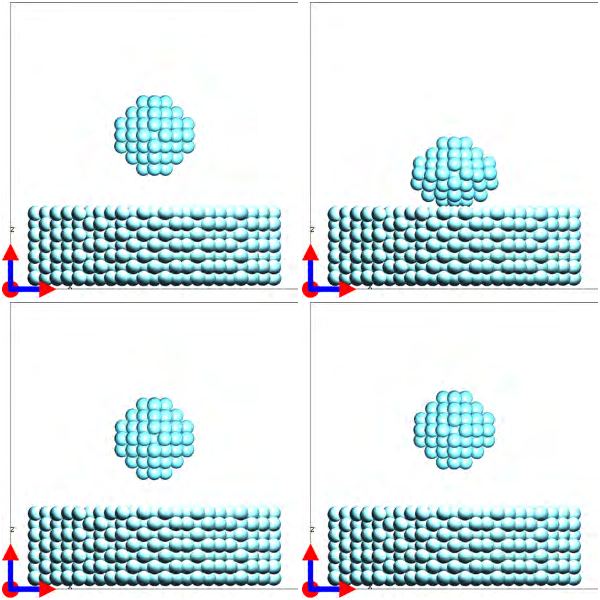
\includegraphics[width=0.46\textwidth]{../manuscrito/figuras_2012_original/fig5_montage.png}\\
\footnotesize Fig.~5 del capítulo ($h_0=11.03\,\sigma$)
\column{0.52\textwidth}
\centering
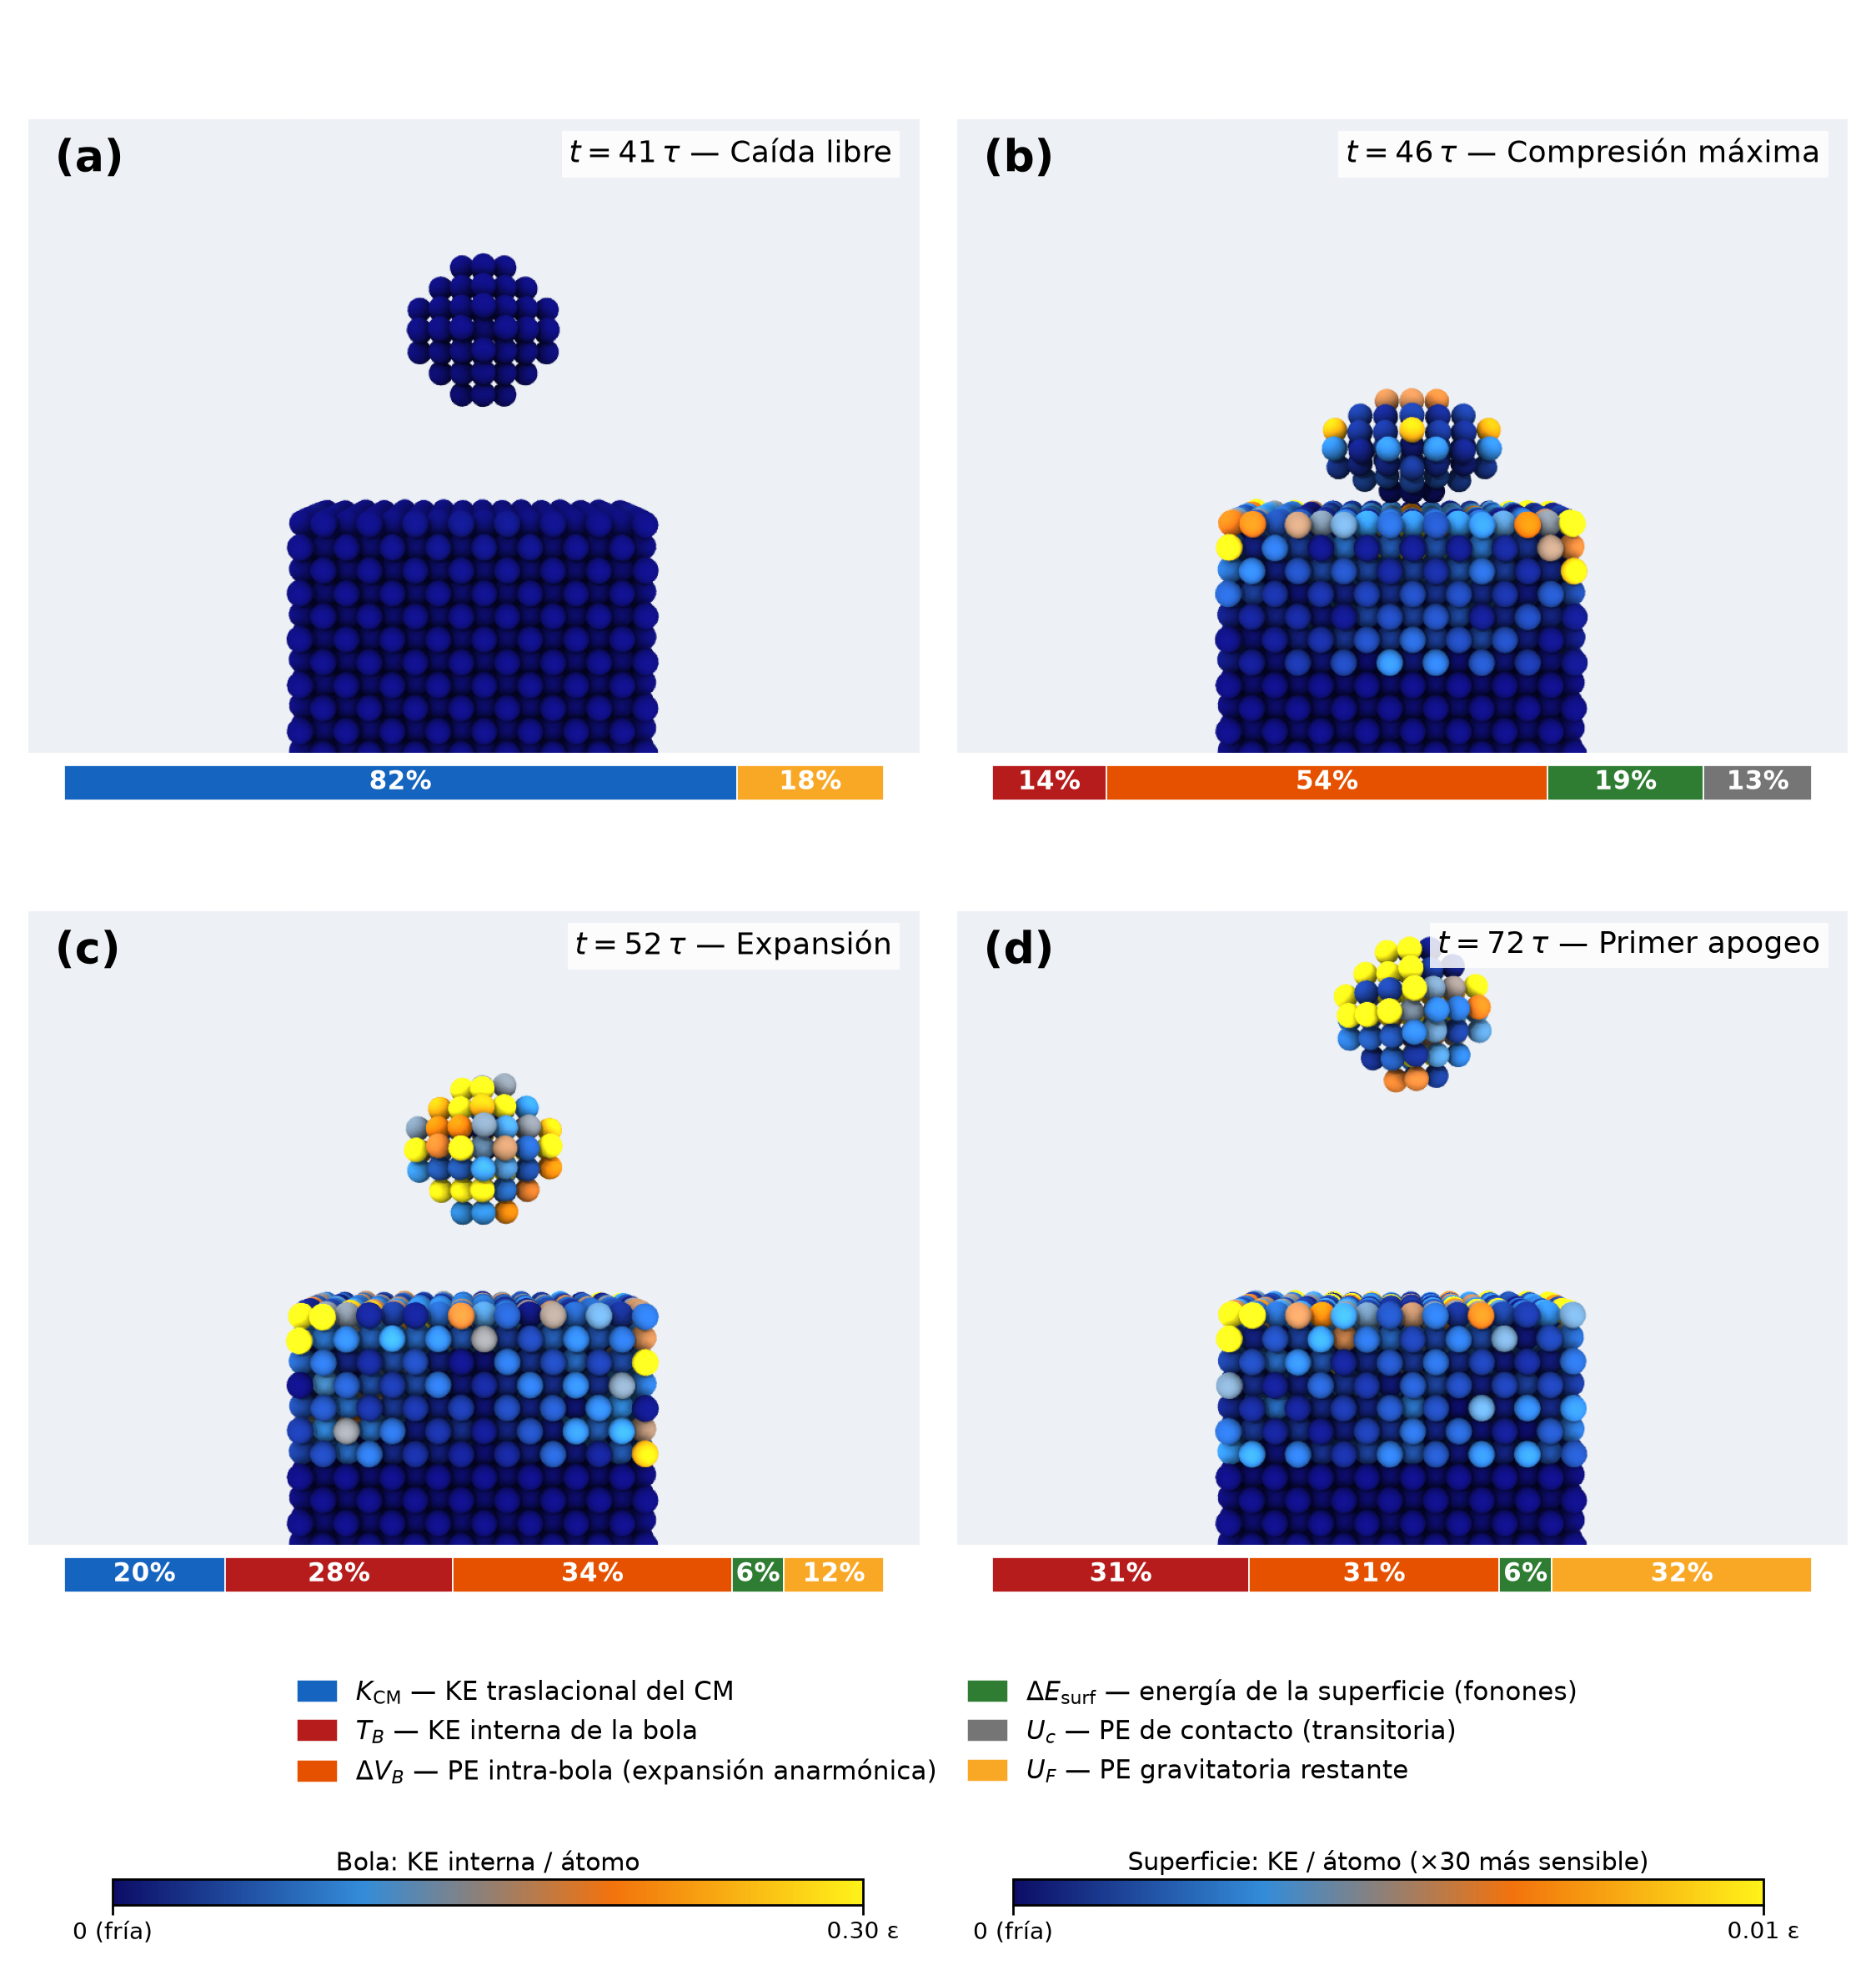
\includegraphics[width=0.56\textwidth]{../figuras_rbef/fig_sequence.png}\\
\footnotesize Nuestra reproducción: $h_0=28.15\,\sigma$, $N=79$ exacto
(\texttt{in.bounce\_cluster})
\end{columns}
\footnotesize
\textbf{6 barras, no 8:} agrupamos $K_S,T_S,V_S\to\Delta E_{\rm surf}$
(verde); $U_c$ (gris) es solo energía \emph{transitoria} visible durante
el contacto. En el apogeo (d), $K_{\rm CM}\to0$ y
$\alpha_{\rm cm}\!=\!U_F/E_0$ (amarillo), $\alpha_{T_B}\!=\!T_B/E_0$
(rojo), $\alpha_{\Delta V_B}\!=\!\Delta V_B/E_0$ (naranjo),
$\alpha_{\rm surf}\!=\!\Delta E_{\rm surf}/E_0$ (verde):
$31\%+31\%+6\%+32\%=100\%$.
\end{frame}

% -----------------------------------------------------------------------------
\begin{frame}{Alturas de rebote sucesivas}
\begin{columns}[T]
\column{0.42\textwidth}
\centering
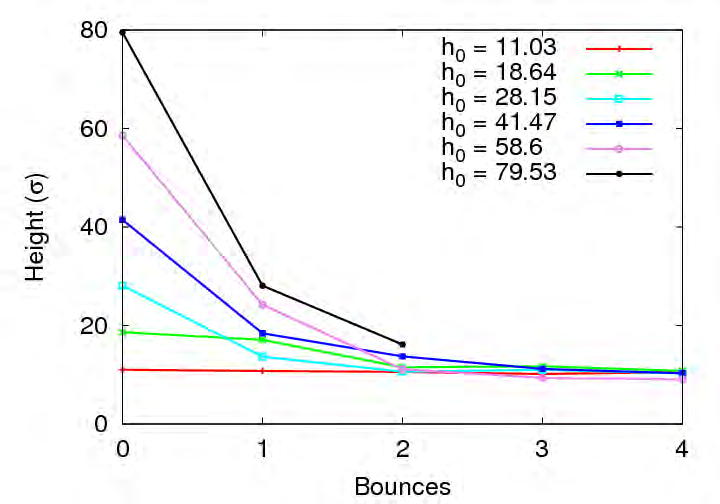
\includegraphics[width=0.6\textwidth]{../manuscrito/figuras_2012_original/fig7_final.png}\\
\footnotesize Fig.~7 del capítulo (hasta el 4\textsuperscript{to} rebote)
\column{0.54\textwidth}
\centering
\includegraphics[width=0.7\textwidth]{../../data/outputs/terminado/reprod_2012/fig_R1_alturas.pdf}\\
\footnotesize Nuestra reproducción (hasta el 25\textsuperscript{to} rebote)
\end{columns}
\begin{alertblock}{\small Hallazgo concreto revisando los logs}
\small
El capítulo fija $M_B=79\,M$, pero reproducir \emph{su misma receta}
(\texttt{create\_atoms region sphere}) da $\mathbf{N=83}$ para
$h_0=11.03\,\sigma$ y $\mathbf{N=84}$ para $h_0=79.53\,\sigma$: el corte
esférico no fija $N$, depende de dónde cae el centro respecto de la red FCC.
\end{alertblock}
\end{frame}

% -----------------------------------------------------------------------------
\begin{frame}{¿Por qué cada altura da un \texorpdfstring{$N$}{N} distinto?}
\begin{itemize}
    \item No es una decisión de diseño --- es un \textbf{efecto
    colateral} de cómo \texttt{in.bounce\_reprod} posiciona la bola.
    \item El centro de la esfera se calcula como
    \texttt{z\_ball\_cm = z\_surf\_top + h0}: depende de $h_0$.
    \item Cada $h_0$ desplaza el centro una cantidad distinta respecto
    del sitio de red FCC más cercano --- y la esfera de radio fijo
    $2.64\,\sigma$ atrapa un número distinto de átomos según cuánto de
    ese desplazamiento ``sobra'' entre capas de la red.
    \item Por eso el resto del proyecto usa \texttt{in.bounce\_cluster}
    con cúmulos armados por \textbf{capas esféricas FCC completas},
    minimizados aparte: $N$ deja de depender de $h_0$ por construcción.
\end{itemize}
\end{frame}

% -----------------------------------------------------------------------------
\begin{frame}{Estructura de la bola: \texorpdfstring{$g(r)$}{g(r)}}
\begin{columns}[T]
\column{0.5\textwidth}
\centering
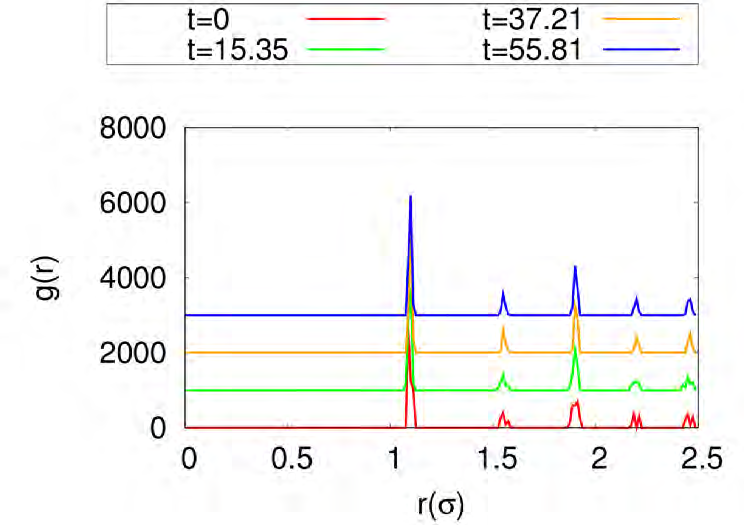
\includegraphics[width=0.32\textwidth]{../manuscrito/figuras_2012_original/fig8_final_000.png}%
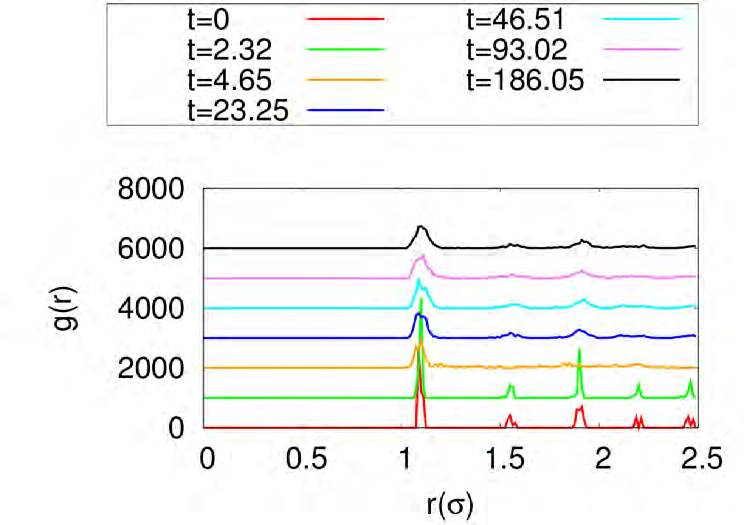
\includegraphics[width=0.32\textwidth]{../manuscrito/figuras_2012_original/fig8_final_002.png}%
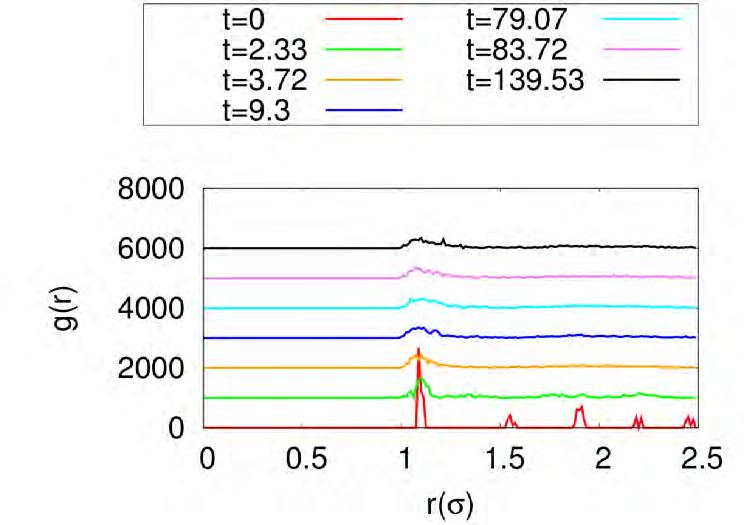
\includegraphics[width=0.32\textwidth]{../manuscrito/figuras_2012_original/fig8_final_005.png}\\
\footnotesize Fig.~8 del capítulo: $h_0=11.03,\,28.15,\,79.53\,\sigma$
\column{0.48\textwidth}
\centering
\includegraphics[width=\textwidth]{../../data/outputs/terminado/reprod_2012/fig_gr_ball.pdf}\\
\footnotesize Nuestra reproducción, mismas tres alturas
\end{columns}
\medskip
\footnotesize
\begin{tabular}{@{}lll@{}}
\toprule
$h_0$ & Capítulo 2012 (Fig.~8) & Nuestra reproducción \\
\midrule
$11.03\,\sigma$ & vecinos 2\textsuperscript{do}/3\textsuperscript{er} sobreviven & ídem: \textbf{FCC conservado} \\
$28.15\,\sigma$ & picos se ensanchan, no colapsan & ídem: \textbf{FCC deformado} \\
$79.53\,\sigma$ & solo sobrevive el 1\textsuperscript{er} pico & ídem: \textbf{FCC $\to$ amorfo} \\
\bottomrule
\end{tabular}
\medskip

\centering\small Mismo umbral de fusión, panel por panel, en dos códigos
de MD independientes --- validación cruzada fuerte del resultado físico.
\end{frame}

% -----------------------------------------------------------------------------
\begin{frame}{Evolución temporal de las energías}
\begin{columns}[T]
\column{0.48\textwidth}
\centering
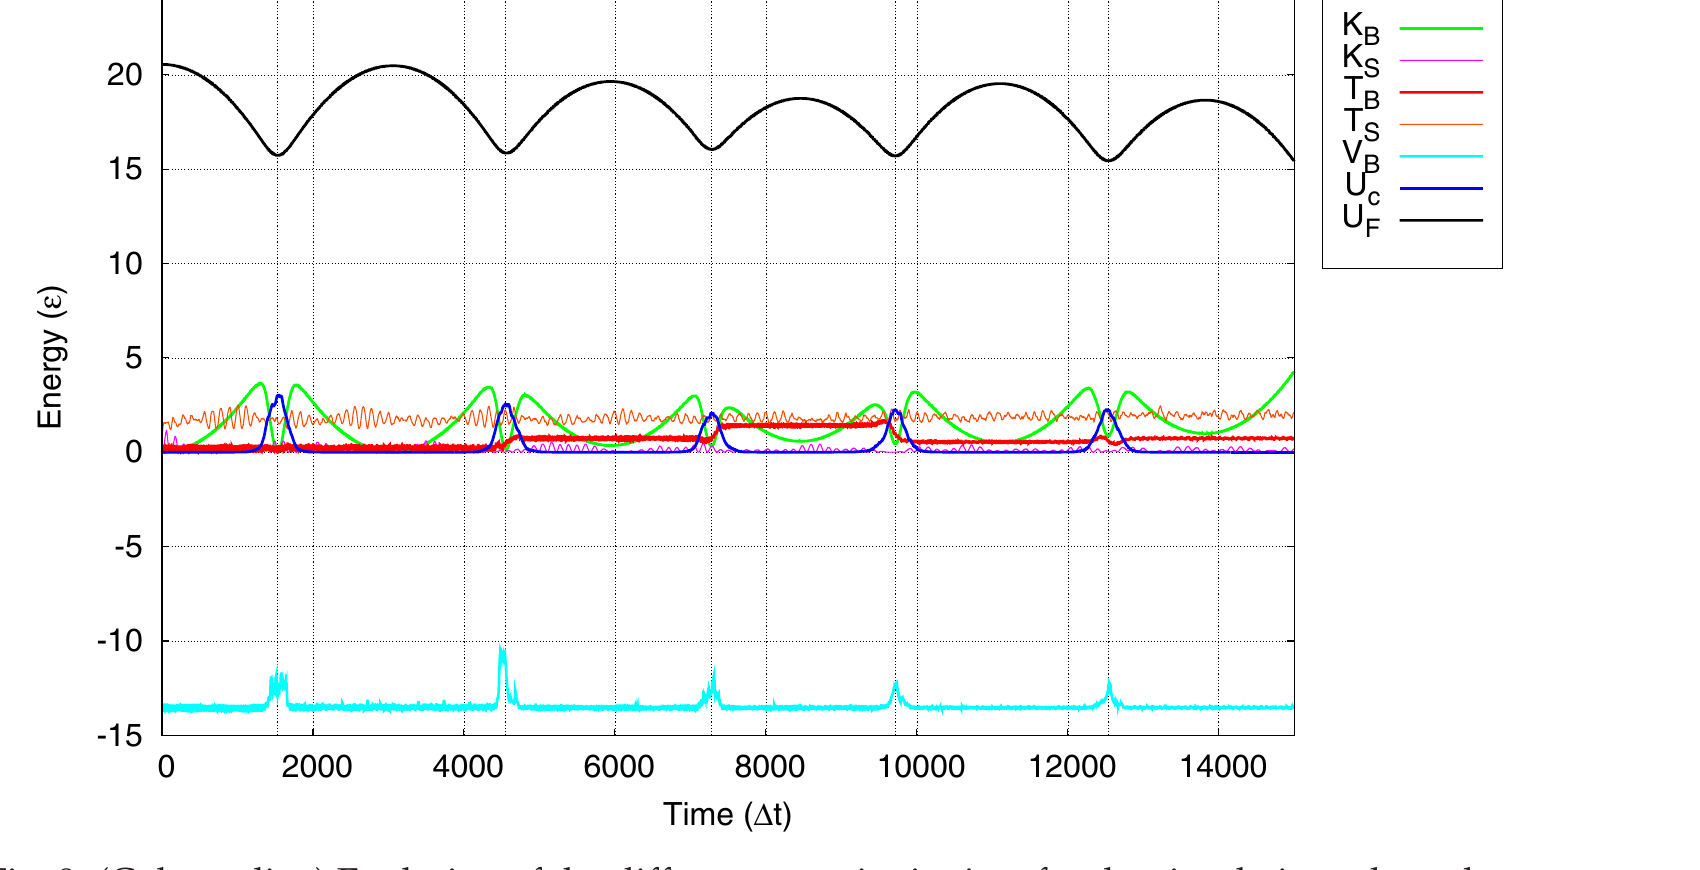
\includegraphics[width=0.78\textwidth]{../manuscrito/figuras_2012_original/fig9_final.png}\\
\footnotesize Fig.~9 del capítulo, $h_0=11.03\,\sigma$ (eje en $\Delta t$)
\column{0.48\textwidth}
\centering
\includegraphics[width=0.78\textwidth]{../../data/outputs/terminado/reprod_2012/fig_R2_energia_h0_11.03.pdf}\\
\footnotesize Nuestra reproducción (eje ya convertido a $\tau$)
\end{columns}
\footnotesize Mismos picos de $K_B$ con mínimos en $K_B=0$, y el mismo
intercambio no monotónico $T_B\!\to\!K_B$ entre el 2\textsuperscript{do}
y 3\textsuperscript{er} rebote que señala el propio capítulo.
\begin{block}{\footnotesize ¿Y la suma de todas las energías?}
\footnotesize
La suma de las 8 energías debería ser \textbf{constante} (sistema
cerrado, sin termostato). En esta corrida temprana (previa al ajuste
\texttt{pair\_modify shift yes}) deriva $\sim5$--$6\%$ de $E_0$ tras 11
rebotes --- la razón medida detrás de agregar ese ajuste (documentado en
\texttt{borrador\_rbef\_v2.tex}).
\end{block}
\end{frame}

% -----------------------------------------------------------------------------
\begin{frame}{Qué mejoramos, y por qué era necesario}
\begin{itemize}
    \item \textbf{Cúmulos de $N$ exacto:} capas esféricas FCC completas +
    minimización, en vez de \texttt{create\_atoms region sphere} ---
    responde directamente al hallazgo $N=83/84$ de la diapositiva anterior.
    \item \textbf{Canal $\alpha_{\rm surf}$ de pleno derecho:} el capítulo
    concluye que $K_S,T_S,V_S$ ``no aportan información'' para su caso de
    baja energía; a velocidades de impacto altas, nuestros datos muestran
    que $\alpha_{\rm surf}$ \textbf{sí} crece y se vuelve comparable a los
    otros canales.
    \item \textbf{Barras de error:} el capítulo reporta una corrida por
    altura; nosotros promediamos 5 orientaciones iniciales por cada
    $(N,h_0)$ --- 210 corridas en total.
    \item \textbf{Barrido en $N$ y reformulación de la equipartición:}
    $N_c^{\rm ef}\approx25\pm8$ constante --- próximas dos láminas.
\end{itemize}
\end{frame}

% -----------------------------------------------------------------------------
\begin{frame}{Barras de error: qué se promedia exactamente}
\begin{itemize}
    \item Para cada par $(N,h_0)$ fijo, el cúmulo (mismos átomos, misma
    geometría FCC interna) se \textbf{rota en un ángulo aleatorio} antes
    de soltarlo sobre la superficie --- 5 orientaciones distintas por
    cada $(N,h_0)$.
    \item Se corre la simulación completa para cada orientación y se
    calculan los 4 canales $\alpha_i$ de cada una por separado.
    \item La barra de error es la \textbf{desviación estándar entre esas
    5 corridas}: cuantifica cuánto importa, para el mismo impacto
    nominal, la orientación relativa del cúmulo respecto de la red de la
    superficie --- variabilidad real del sistema, no ruido numérico.
    \item El capítulo 2012 corre una sola orientación por altura, así que
    no hay forma de saber, a partir de él, si sus números son
    representativos o una muestra particular.
\end{itemize}
\end{frame}

% -----------------------------------------------------------------------------
\begin{frame}{¿Qué es \texorpdfstring{$N_c^{\rm ef}$}{Nc\_ef}?}
\begin{itemize}
    \item La bola tiene $3N-3$ modos internos de vibración. Si la energía
    \textbf{disipada} (la que no vuelve al CM, $1-\alpha_{\rm cm}$) se
    reparte por equipartición entre esos modos y los de la porción de
    superficie que participó del contacto, la fracción que se queda en la
    bola es
    \[
    f_{\rm ball}\equiv\frac{\alpha_{\rm bola}}{\alpha_{\rm bola}+\alpha_{\rm surf}}
    =\frac{3N-3}{3N-3+3N_c^{\rm ef}}.
    \]
    \item $N_c^{\rm ef}$ es, por definición, el \textbf{número efectivo de
    osciladores de superficie} que compiten con los $3N-3$ de la bola por
    esa energía disipada --- no el número de átomos que se mueven, sino
    cuántos modos ``cuentan'' en el reparto neto.
    \item Midiendo $f_{\rm ball}(N)$ para $N=2,\ldots,87$ e invirtiendo la
    fórmula, se obtiene $N_c^{\rm ef}\approx25\pm8$, \textbf{constante}
    (no crece con $N$).
    \item Consecuencia directa: $f_{\rm ball}\to1$ cuando $N\to\infty$
    (no $\to\tfrac12$, como predecía el argumento ingenuo con
    $N_c=N$) --- una bola grande se queda con casi toda la energía que no
    devuelve al CM.
\end{itemize}
\end{frame}

% -----------------------------------------------------------------------------
\begin{frame}{Por qué \texorpdfstring{$N_c^{\rm ef}$}{Nc\_ef} es tan chico: tres escalas distintas}
\begin{columns}[T]
\column{0.56\textwidth}
\centering
\includegraphics[width=0.92\textwidth]{../figuras_rbef/fig_Nc_escalas.pdf}
\column{0.42\textwidth}
\footnotesize Medido en el dump ($v_{\rm imp}\approx1.47$):
\medskip

\footnotesize
\begin{tabular}{@{}ll@{}}
$N_c^{\rm ef}\approx25$ & neto \\[1pt]
$\ll N_c^{\rm geom}\approx45$--$90$ & huella \\[1pt]
$\ll N_c^{\rm part}\approx300$--$410$ & KE alto \\
\end{tabular}
\end{columns}
\footnotesize
Cientos de átomos se mueven \emph{transitoriamente} ($N_c^{\rm part}$),
en una huella geométrica de $\sim$45--90 vecinos ($N_c^{\rm geom}$) ---
pero casi toda esa energía \textbf{vuelve} al despegar la bola, porque la
superficie es casi elástica. Lo que se queda neto corresponde a solo
$\sim$25 modos: eso es $N_c^{\rm ef}$, y es el que gobierna $f_{\rm ball}(N)$.
\end{frame}

% -----------------------------------------------------------------------------
\begin{frame}{Resumen}
\begin{alertblock}{La reproducción es sólida}
Cuatro figuras cuantitativas independientes del capítulo 2012 coinciden,
panel por panel, con nuestra reproducción en \lammps{}.
\end{alertblock}
\begin{block}{Y encontramos algo real al hacerla}
El corte esférico no da $N$ exacto ($83$/$84$ en vez de $79$) --- la
motivación concreta, medible, detrás de reconstruir los cúmulos por capas
FCC completas y de todo el barrido en $N$ que sigue.
\end{block}
\medskip
\centering\small Notas completas:
\texttt{docs/manuscrito/comparacion\_energias\_2012.tex} y
\texttt{comparacion\_figuras\_2012.tex}.
\end{frame}

\end{document}
